\chapter{Results}
\label{cha:result}
Experiments \fix{TODO}
\section{CoDA-PCA Microbiome data}
Smallish for both dimensions, uses OTUs at genus level

Still no improvement over baseline using end to end. Even with larger sample size (1000), performance is at best the same, often much lower.  

\section{RUG}
New microbiome results, using species level  
- Poor performance, can't do better than chance
- Why?: Sheer depth of connections needed in 'fat' matrices to map them to a lower dimension. The small sample size does not allow for enough information for the network to establish meaningful relationships between the input, low level representation and the output. 
- Preprocessing with dim reduction works better because the dimensionality reduction algorithms are fixed, and there is no need to learn them unlike in the network.
- Can see from 2D/3D plots there is not enough information in these dimensions to meaningfully distinguish classes. Also note the different representations of PCA and CoDA-PCA

A lot of modern results are of this 'fat' form, given the small sample sizes and large diversity in microbiome species. To improve performance/reduce size it may make sense to do analysis at the genus or higher level. 

https://microbiomedb.org/mbio/app/ other sources if needed

%\section{Direct Cost}\
%\label{sec:direct_cost}

%Here is the example to show how to include a figure. %Figure~\ref{fig:cost}
%includes two subfigures (Figure~\ref{fig:zerocost}, and %Figure~\ref{fig:zerobus});

%\begin{figure*}
%  \label{fig:cost}
%  \subfigure[Fraction of cycles spent on %zeroing\label{fig:zerocost}]{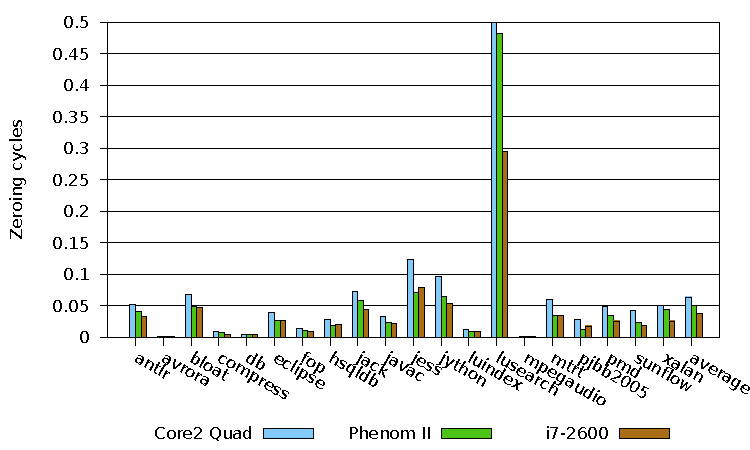
\includegraphics[width=\columnwidth]{f%igs/zerocost_intel.pdf}}
%  \subfigure[BytesZeroed / %BytesBurstTransactionsTransferred\label{fig:zerobus}]{\includegraph%ics[width=1.0\columnwidth]{figs/zerobus_core.pdf}}
%  \caption{The cost of zero initialization}
%\end{figure*}


\section{Summary}
